\documentclass[10pt,twocolumn,letterpaper]{article}

% Миний хувийн зүйлс
\usepackage{booktabs}
% \usepackage{caption}
% \captionsetup[table]{skip=8pt}   % Зөвхөн хүснэгтүүдэд нөлөөлнө
\usepackage{stfloats}  % Үүнийг эхэнд нь нэмнэ үү
\usepackage{float}
\usepackage[T2A]{fontenc}

% \usepackage{fontspec}
\usepackage[english]{babel}

% load Lao via babelprovide, turn on "onchar=ids" for automatic shaping
\babelprovide[import,onchar=ids fonts]{mongolian}

% main (rm) font for Latin
\babelfont{rm}{Noto Serif}
% alternate (sans-serif) font for Latin
\babelfont{alt}{Lato}

% Lao text in Noto Serif Lao at 1.2× scale
\babelfont[mongolian]{rm}{Noto Serif}
\babelfont[mongolian]{sf}{Noto Serif}
% Lao text in Noto Serif Lao for the alt family too
\babelfont[mongolian]{alt}{Noto Serif}

\usepackage{cvpr}
\usepackage{times}
\usepackage{epsfig}
\usepackage{graphicx}
\usepackage{amsmath}
\usepackage{amssymb}

% Энд бусад багцуудаа оруулна уу, hyperref-ээс өмнө.

% Хэрвээ та hyperref-г комментаар авч дараа нь буцааж идэвхжүүлбэл,
% устгах шаардлагатай

% egpaper.aux-г дахин ажиллуулахаас өмнө.  (Эсвэл эхний латекс ажиллуулалтын үед 'q'-г дараад, дуусгаж байгаарай, тэгээд тодорхой болно.)
\usepackage[breaklinks=true,bookmarks=false]{hyperref}

\makeatletter
\def\cvprsubsection{\@startsection {subsection}{2}{\z@}
    {8pt plus 2pt minus 2pt}{6pt}{\bfseries\normalsize}}
\makeatother

\cvprfinalcopy % *** Эцсийн хувилбарыг илгээхэд энэ мөрийг идэвхжүүлнэ үү

\def\cvprPaperID{****} % *** CVPR өгүүллийн дугаарыг энд оруулна уу
\def\httilde{\mbox{\tt\raisebox{-.5ex}{\symbol{126}}}}

% Илгээх горимд хуудсууд дугаарлагдсан, эцсийн хувилбарт дугааргүй байна
%\ifcvprfinal\pagestyle{empty}\fi
\setcounter{page}{1}
\begin{document}

%%%%%%%%% ГАРЧИГ
\title{ECDO Мэдээлэлд Суурилсан Анхан Шатны Хэсэг 1/2: Экзотермик Цөм-Бүрхүүлийн Салалтын Dzhanibekov Хэлбэлзэл (ECDO) “Дэлхийн Эргэлт” Онолын Одоогийн Ойлголт}

\author{Жүнхо\\
2025 оны хоёрдугаар сард хэвлэгдсэн\\
Вэбсайт (Эндээс өгүүллүүдийг татах): \href{https://sovrynn.github.io}{sovrynn.github.io}\\
ECDO Судалгааны Сан: \href{https://github.com/sovrynn/ecdo}{github.com/sovrynn/ecdo}\\
{\tt\small junhobtc@proton.me}
% Зохиогчид бүгд нэг байгууллагад харьяалагддаг нийтлэлд,
% дараах мөрүүдийг хаалтын ``}'' тэмдэг хүртэл орхино.
% Нэмэлт зохиогчид болон хаягуудыг ``\and''-аар нэмж болно,
% яг хоёр дахь зохиогчийн нэгэн адил.
% Зай хэмнэхийн тулд имэйл хаяг эсвэл нүүр хуудсыг нэгийг нь сонгож хэрэглэнэ үү 
% \and
% xxx
% Байгууллага2\\
% Байгууллага2-ын хаягийн эхний мөр\\
% {\tt\small secondauthor@i2.org}
}

\maketitle
%\thispagestyle{empty}

%%%%%%%%% ХУРААНГУЙ
\begin{abstract}
2024 оны тавдугаар сард “Ёс зүйн Скептик” нэртэй нууц нэртэй онлайн зохиогч \cite{0} “Экзотермик Судал (Цөм-Бүрхүүл)-ийн Салангид Жанибеков Осцилляцийн онол” (ECDO) \cite{1} хэмээх шинэлэг онолыг хуваалцсан. Энэ онолд Дэлхий эргэлтийн тэнхлэг нь өмнө нь гэнэт, гамшигт өөрчлөлтөд орж, эргэлтийн инерциэс болж далай тэнгисүүд тивүүд рүү халин асгарч асар их үерлэлт үүсгэж байсан гэж үздэг. Түүнчлэн дахин ийм үйл явдал болох магадлалтайг илтгэх геофизикийн тайлбар процесс болон баримтыг танилцуулдаг. Иймэрхүү сүйрлийн үер, дэлхийн сүйрлийн таамаглал шинэ зүйл биш боловч, ECDO онол шинжлэх ухаанч, орчин үеийн, олон салбарын, өгөгдөлд суурилсан хандлагаараа онцгой анхаарал татаж байна.

This paper is the first part of a two-part condensed summary of six months of independent research \cite{2,20} into the ECDO theory. It highlights three key points:

\begin{flushleft}
\begin{enumerate}
    \item ECDO-тэй төстэй 'Дэлхий эргэх' үзэгдэл нь хүн төрлөхтний сүүлийн үеийн түүхэнд олон удаа тохиолдсон бөгөөд үүнийг үерийн домог болон эх газруудаар дэлгэрсэн үертэй холбоотой геологийн шинж тэмдгүүд нотолдог.
    \item Өмнөх Дэлхийн эргэлтийн ерөнхий чиглэл болон хэмжээ (хүч)-ийг тодорхойлж болно.
    \item Сүүлийн үеийн соронзон болон геофизикийн мэдээлэл нь дахин нэг Дэлхийн эргэлт ойртож байж магадгүйг, мөн уур амьсгалын өөрчлөлт нь хүний үйл ажиллагаанаас бус харин Дэлхийн дотоод гүнд болсон өөрчлөлтөөс шалтгаалж болохыг харуулж байна.
\end{enumerate}
\end{flushleft}

Мөн түүнчлэн, энэхүү өгүүлэлд ECDO онолд дэвшүүлсэн “Дэлхийн эргэлт”-ийн шалтгаан болсон физикийн үндсийг авч үзнэ.

Энэ өгүүлэлд би зөвхөн бодит өгөгдөлд төвлөрч, таамаглал ихтэй ч итгэл үнэмшил төрүүлэх хэсгүүдийг зайлсхийж, хүн төрөлхтний хувьд цаашид яаралтай судлах шаардлагатай сэдэв болохыг онцлон тэмдэглэв.
\end{abstract}

%%%%%%%%% BODY TEXT
\section{Удиртгал}

Их үерийн тухай түүх шинэ зүйл биш - үнэндээ энэ нь дэлхийн бүх голлох соёл иргэншилд, бүх соёлын өлгийд байдаг. 267 үерийн түүхийн эмхэтгэл (Зураг \ref{fig:1})\cite{3}-ийг зураглаж үзвэл хүн амьдардаг бараг бүх бүс нутагт үерийн түүхүүд байдаг болохыг харуулдаг.
% \begin{figure}[h]
% \begin{figure}[b]
\begin{figure}[h]
\begin{center}
% \fbox{\rule{0pt}{2in} \rule{0.9\linewidth}{0pt}}
   \includegraphics[width=1\linewidth]{b.png}
\end{center}
   \caption{Дэлхий даяар үерийн тухай түүхүүдийн байршил \cite{3}.}
\label{fig:1}
\label{fig:onecol}
\end{figure}

Эдгээр үерийн түүхийг илүү анхааралтай судлахад энэ нь энгийн үер биш, харин тивүүдийг бүрэн цэвэрлэсэн сүйрлийн гамшиг дагалдсан үерүүд болох нь харагддаг.

\subsection{Америкийн уугуул иргэдийн гамшгийн түүхүүд}

Америкийн уугуул иргэдийн түүхүүдэд дэлхийн их гамшгийн хамгийн тод өгүүлэмжүүд багтдаг. Баруун хойд Аризонад амьдардаг Хопи омгийнхон, \textit{"..Сотукнанг хий сонгогдсон хүмүүст зориулж шоргоолжны оршин суудаг газар доорх дэлхийг нээхийг шоргоолжнуудад тушаажээ. Тэд аюулгүй газар дор ороход, Сотукнанг ихрийн хоёр, Пёкванхоя болон Палөнгавхоя хоёрыг дэлхийн гол тэнхлэгийн хойд ба өмнөд үзүүрт байсан харуулын байрлалыг орхихыг тушаав. \textbf{Ихрүүд харуулын газраа орхиход дэлхийг хянах хүнгүй болж, дэлхий тэнцвэргүй болж, галзуу юм шиг эргэж, хоёр удаа хөрвөв.} Уулс их дуу чимээтэй далайд уналаа, тэнгис, нуурнууд газраар халин асгарав; мөн дэлхий хүйтэн, амьгүй огторгуйд эргэх үед цэвдэг мөс болж хөлдөв"} \cite{4} гэж өгүүлдэг.

Эдгээр түүхийн ихэнх нь үерийн цар хүрээг маш нарийн тодорхойлон өгүүлж, далай тэнгисүүд хамгийн өндөр уулсын оргилыг эс тооцвол бүгдийг нь живүүлсэн тухай өгүүлдэг. Вашингтон мужид амьдардаг Скокомиш индианчууд, \textit{"Аугаа Сүнс, хүмүүс ба амьтдын ёс бус байдлаас уурлаж, зөвхөн сайн амьтад, нэг сайн хүн болон түүний гэр бүлээс бусдыг газраас зайлуулах шийдвэр гаргажээ. Аугаа Сүнсний заавраар тэр эр хүн үүл рүү сум харваж, дараагийн сумыг тэр сум руу, тэр чигээр нь дахин дахин харваж үүлнээс газар луу суман утас үүсгэв. Сайн амьтад, хүмүүс тэр утсан дээр авирчээ. Муу амьтад ба могой авирч эхлэсэн боловч тэр эр утсыг таслав. \textbf{Дараа нь Аугаа Сүнс олон хоног бороо орж, ус Такахома (Рейниер уул)–ын цасны шугам хүртэл дээш гарчээ.} Бүх муу хүмүүс амьтад живж дуусах үед Аугаа Сүнс бороог зогсоосон, ус удаанаар буурч, сайн хүмүүс амьтад буужээ"} \cite{3} гэж өгүүлдэг. Жишээ болгож хэлэхэд, Рейниер уул нь Вашинтон мужид орших идэвхитэй галт уул бөгөөд оройн өндөр нь далайн түвшнээс дээш 4392.5 метр юм.
Makah овгийн Вашингтоны мужийн үерийн тухай домогт "маш дулаан" устай олон үе шаттай үерийн тухай тодорхой дурдсан байдаг бөгөөд энэ нь энгийн үер байгаагүйг харуулж байна: \textit{"Далай тэнгис толгойг таслахуйц өндөрт мандсан. Тэгээд тэр буцаж, дөрөв хоногийн дараа хамгийн нам түвшиндээ хүрч, Неа буланг хуурай газар болгосон. Дараа нь дахин өсч, уулын оройгоос бусдыг бүгдийг нь усанд автуулсан. \textbf{Өсөх ус маш дулаан байсан.} Завьтай хүмүүс эд хогшлоо ачаад хол хойд зүг рүү авч явсан. Заримынх нь зави модонд хавчуулагдаж олон хүн амиа алджээ. Дөрөв хоногийн дараа тэнгис энгийн байдалдаа эргэж, хүмүүс хойд зүгт хүрч үлдсэн ба тэнд үр удам нь одоо ч амьдардаг"} \cite{3}.

\subsection{Хятадын сүйрлийн тухай домгууд}

Номхон далайн нөгөө эрэгт, өнөөгийн Хятадын соёл иргэншил их үертэй холбоотой үүссэн гэж ярьдаг. МЭӨ 2000 оны орчим үүссэн гэж тооцогддог Шя гүрнийг Юу Их хүн байгуулсан ба тэрээр Гун-Югийн Их үерийг зогсоосон \cite{6}. Түүний үед, \textit{"... гайхамшиг болсон нь арван өдөр нар жаргахгүй байсан, ой шугуй шатсан бөгөөд аймшигтай шавьж бөөнөөр гарсан гэж ярьдаг... Тэнгэрийг хүртэлх өндөр давалгаа Хятадын газар дээр унасан. \textbf{"Ус уулын оргилоос давж, уулын бэл харагдахгүй болсон"}... "Үерийн аюулын усаар сүйрч байна" гэж эзэн хаан хэлэв. "Уудам талбайд уулсыг тэврэн, өндөрлөг газрыг давж, үертэйгээр тэнгэрийг заналхийлж байна." Эзэн хаан уулсын хооронд хавчигдсан усыг гаргах гарц нээхийг бүгдэд даалгасан. Олон жилийн турш ард түмэн тал газар болон хөндийг үерийн усаас чөлөөлөхийн тулд суваг суваг үүсгэн талбайг хатаах гэж ажиллажээ. Олон жилийн туршид хийсэн бүх хүчин чармайлт үр дүнгүй байв. Энэ яаралтай, асар их ажлыг удирдсан сайд Хуаныг бүтэлгүйтсэн гэж цаазаар авчээ... зөвхөн түүний хүү Юу газар нутгийг усаас чөлөөлж чадсан. Энэ ололтыг маш өндөр үнэлсэн тул Юу нь хаан Шуны дараагаар Хятадын эзэн хаан болсон, Шяоугийн анхны залгамжлагч"} \cite{5}.

Зөвхөн Хятад үерлээд зогсоогүй, харин мөн зүг чиг, нар сарны хөдөлгөөнийг дахин хэмжих шаардлагатай болсон нь дэлхийн тэнхлэг өөрчлөгдсөн байж магадгүйг илтгэнэ: \textit{\textbf{"Тэр эзэн хаан Хятадын өөр өөр хэсэгт болон тэр ч байтугай Индохятад руу эрдэмтдийг илгээж, нар мандах ба шингэх чиглэл, оддын хөдөлгөөнийг ажиглон умард, өрнө, дорно, өмнөдийг тогтоохыг даалгасан.} Тэр мөн одон орончдоо улирлын үргэлжлэх хугацааг олох, шинэ хуанли гаргахыг даалгасан... "Тэгээд Яоу [Шяоу] Хэ, Хо нарыг өргөн тэнгэрийг хүндэтгэн, нар, сар, од, ордуудын хөдөлгөөн, төрх байдлыг тооцоолж зурж, улирлуудыг ард түмэнд хүндэтгэлтэйгээр дамжуулахыг тушаав""} \cite{5}.

Хятадын түүхэн дэх гамшгийн тэмдэглэл Шя гүрнээс 훨 өмнө үеэс, гурван эзэн, таван хааны үе хүртэл оршиж байсан юм \cite{7}. Нюва, гурван эзний нэг бөгөөд Хятад түүхийн төвд байдаг бүтээлийн дүр, дэлхий тэнхлэгээ өөрчлөх гамшгийн үед үерийг зогсоосон: \textit{"Хоёр хүчирхэг бурхан хоорондоо маргалдан, тэмцэхээр болжээ. Усны бурхан Гун Гун ялагдаж байгаа гэдгээ ойлгоод, толгойгоо Бужоу уул руу цохижээ, тэрхүү уул нь тэнгэрийг тулж байсан багана байв. \textbf{Багана нурж, тэнгэр баруун хойш, газар зүүн урагш тийш хазайжээ.} Үүнээс болж асар их гамшиг: тасралтгүй гал түймэр, уудам үер, догшин махчин араатнууд гарч ирсэн. Нюва аварга яст мэлхийн хөлийг тайрч унасан баганы оронд ашиглаж, нөхцөл байдал намдаан, тэнгэрийн цуурсан хэсгийг долоон өөр өнгийн чулуугаар бөглөсөн ч тэнгэрийн хазайлтыг бүрэн засаж чадаагүй"} \cite{8}.

\subsection{Европ, Майя, Ойрх Дорнод болон Зүүн Өмнөд Азийн сүйрлийн тухай домгууд}

Энэ өгүүлэлд бүх сүйрлийн домгийг нарийвчлан оруулж багтаах боломжгүй тул бусад онцлох соёлын зарим домгийг товч дурдъя. Грекийн уран зохиолд Деуалион, Огиг, Дарданус гэсэн гурван үерийн домог байдаг \cite{9,10}. Эхний тохиолдолд, \textit{"Есөн хоног үерлэсний дараа дэлхий сүйрч, авралын хөлөг Парнассын уулын орой дээр зогссон"}, уг уулын оргил 2,457 метр өндөртэй \cite{11}. Майя бичиглэлд өнөөгийн нарнаас өмнө дөрвөн өөр нар байсан, дөрөв дэх нар болох Калчиутликүгийн үе дуусахдаа дэлхийг бүрэн сүйрүүлсэн үер болж, МЭӨ 3100 онд өнөөгийн тав дахь нар мэндэлсэн гэж үздэг \cite{12}. Ойрхи Дорнодод Библийн он тоолдолд алдартай Ноагийн үер, Вавилоны шүлэг болох Гильгамешийн туульд ижил төстэй домог бий \cite{13}. Зүүн Өмнөд Азийн соёлд ч үерийн домог элбэг - жишээ нь Индонезийн От Данумынхан, \textit{"Нэгэн асар их үер олон хүнийг живүүлсэн. Цөөн хэдэн хүн уснаас давсан ганц уулын орой руу завиар зугтаж амьд гарсан. Тэд гурван сарын турш тэнд амьдарч, үер намдмагц доош буужээ"} \cite{3}. Тэдний амьдардаг Борнео арал 4,095 метр оргилтой юм.

\begin{figure*}[b]
\begin{center}
% \fbox{\rule{0pt}{2in} \rule{.9\linewidth}{0pt}}
\includegraphics[width=1\textwidth]{marine.jpg}
\end{center}
   \caption{Далайн (усан доорх) чулуужсан олдвор, давст ус болон давсны талбай/уул уурхайн дэлхийн зураг \cite{15,16,86,87}.}
   \label{fig:2}
\end{figure*}

\subsection{Катастрофын тухай түүхийн статистик шинжилгээ}

Илэрхий, эдгээр түүхүүд нь их үерийн хамтаар бусад төрлийн гамшигт геофизикийн хүчнүүд давхар тохиолдсон болохыг дүрслэн өгүүлдэг. 117 катастрофын тухай түүхийн (Хүснэгт \ref{tab: 1}) шинжилгээгээр их үерийн хажуугаар галан шуурга, газрын гадаргын өөрчлөлт, дэлхийн эргэлтийн өөрчлөлт хамт тохиолдсон гэж олон тохиолдолд тэмдэглэгдсэн байдаг \cite{14}:

\begin{table}[ht]
\begin{center}
\renewcommand{\arraystretch}{1.2}  % Optional, to increase row spacing
\begin{tabular}{|l|c|c|}
\hline
\textbf{Катастрофын төрөл} & \textbf{Тоо} & \textbf{Давтамж (\%)} \\
\hline\hline
Их үер/усны үер           & 84 & 71.79 \\
Галан шуурга/галын гамшиг & 39 & 33.33 \\
Гадаргын өөрчлөлт         & 29 & 24.79 \\
Сүүлэг оддын эмх замбараагүй байдал & 15 & 12.82 \\
Тэнгэр нурсан              & 15 & 12.82 \\

Prolonged darkness      & 14 & 11.97 \\
Устаж үгүй болсон газрууд ба нуурнууд    & 12 & 10.26 \\
Циклон салхи          & 10 & 8.55  \\
Тэнхлэгийн/эргэлтийн өөрчлөлт & 9 & 7.69  \\
Буцалж буй гол, нуур, далай & 8 & 6.84 \\
\hline
\end{tabular}
\end{center}
\caption{Өгүүллэгүүдэд гардаг гамшгийн үр дагаврын тохиолдлууд}
\label{tab: 1}
\end{table}

Дэлхийн өнцөг булан бүрийн бие даасан олон соёлд үерийн тухай өгүүллэг онцгой нарийвчлалтайгаар гарч ирдэг нь, түүнчлэн бусад сүйрлийн үзэгдлийн хувь заяа ижил төстэй өгүүллэгүүдтэй таарч байгаа нь эдгээр үерийн өгүүллэгүүд нь үнэхээр болсон гамшгийн шууд дүрслэл байж болзошгүйг илтгэнэ.

\section{Далайн үерийн физик нотолгоо}

Үерийн өгүүллэгийг нотолсон янз бүрийн хэлбэрийн физик нотолгоо нь дэлхийн эх газрын гадаргуу дээр өргөн тархсан далайн усанд автсан шинжүүд юм. Хамгийн шууд хэлбэрийн нотолгоонд давс (давстай ус, давсны талбай, давсны уурхай) болон далайн (далайн гаралтай) чулуужсан үлдэгдэл буюу олдвор ордог бөгөөд эдгээр нь дэлхийн эх газрын ихэнх хэсгийг хамарсан байдаг. Зураг \ref{fig:2}-т давстай ус (цэнхэр), давсны талбай ба уурхай (бор), болон далайн чулуужсан үлдэгдэл \cite{15,16,86,87}-ийн тархалтыг харуулсан бөгөөд эдгээр нь далайн үерийн ул мөрийн хэмжээг илтгэнэ.

Давстай ус агуулсан хамгийн сонирхолтой газруудын нэг нь Төвдийн Хималайн өндөрлөг болон Өмнөд Америкийн Андын нуруу юм; эдгээр газар дунджаар 4000 метр өндөрт орших бөгөөд эхнийх нь Зураг \ref{fig:3}-д үзүүлэгдсэн. Төвдийн үерийн домогт, \textit{"\textbf{Төвд бараг бүхэлдээ усанд автаж}, туйлд нь гарсан хүмүүсийг бурхан Гя өрөвдөн, усыг Бенгалаар урсгаж, хүмүүсийг соёлжуулах гэж багш нар илгээсэн. Учир нь тэд тэр үеэс өмнө сармагчингаас илүү дээр биш байсан"} \cite{3} хэмээн өгүүлдэг. Перугийн домогт уул үүсэх болон уулын оройг хамарсан үер зэрэгцэн тохиолдсон тухай өгүүлдэг: \textit{"Хоничны зургаан хүүхэдтэйгээ хамт боломжит бүхий л хүнс болон хоньдоо авч, маш өндөр Анкасмарка уулын оройд гарсан. \textbf{Үерийн ус нэмэгдэхэд, уул ч мөн өндөрсөж, түүний орой усанд автахгүй байсан, дараа нь уул усаар буцаад доошилсон.} Үерийн дараа зургаан хүүхэд аймгийг дахин хүн амьтнаар засан суурьшсан"} \cite{3}.
\begin{figure}[t]
\begin{center}
% \fbox{\rule{0pt}{2in} \rule{0.9\linewidth}{0pt}}
   \includegraphics[width=1\linewidth]{tibet.jpg}
\end{center}
   \caption{Гималайн газрын гадаргын зураг—давстай ус (циан өнгөтэй), хатсан давс (цагаан), далайн чулуужсан амьтдын үлдэгдэл (улаан) \cite{15,16,86,87}.}
\label{fig:3}
\label{fig:onecol}
\end{figure}

Геологийн уламжлалт сургуулийн үзэл бодлоор иймэрхүү гаж үзэгдлүүд—давс болон далайн чулуужсан амьтан—дараалан олон сая жилийн турш болсон урт удаан үйл явцаар тайлбарлагддаг. Гэвч хүн төрөлхтний үерийн тухай домгууд энэ сэтгэлгээнд эргэлзэхэд хүргэнэ. Хэрэв далай үнэхээр эх газрыг нөмөрч байсныг бодит гэж үзвэл, өндөрлөг газрын өргөн уудам нутагт давстай ус, далайн чулуужсан ул мөрийг олж илрүүлэх нь яг л бидний хүлээх үр дүн байх ёстой.

\begin{figure*}[t]
\begin{center}
\includegraphics[width=0.85\textwidth]{khafre.jpg}
\end{center}
   \caption{Түр хугацаанд далайн түвшин нэмэгдсэнээс болж ялгаатай, хээтэй карстын элэгдэл үүссэн байдлын бүдүүвч диаграмм \cite{27}.}
\label{fig:4}
\end{figure*}
\subsection{Нэмэлт Физикийн Этгээд Явдлууд}

Жигд үйл явцын онолоор тайлбарлах боломжгүй олон төрлийн этгээд үзэгдлүүд бий. Мянга мянган жилийн дараа ч идэж болохуйц махтай, шаварт булсан, яг зэрэг хөлдсөн мамонтууд \cite{17,18,19}, Хойд Америкийг хамарсан 2.4 сая км$^2$ талбайг бүрхсэн, маш том хүрээний хөндлөн давхаргатай хурдсын тоноглолууд \cite{21}, мегахүчний долгионт газрын тогтоц \cite{22}, хэдэн зуун км-н холоос гаралтай, уулын оргилууд дээр орших үл мэдэгдэх том чулуу \cite{23,26} зэрэг нь орчин үеийн жигд үйл явцын геологичид “урт хугацааны явцад болсон үйл явц” гэх нийтлэг тайлбараар хялбархан тойрч өнгөрдөг үзэгдлүүдийн зөвхөн зарим нь. Ийм этгээд үзэгдлүүдийг гамшигт геофизикийн хүчээр хамгийн сайн тайлбарлаж болох бөгөөд энэ өгүүллийн хоёрдугаар хэсэгт дэлгэрэнгүй авч үзнэ.

Мөн, дэлхийн палеомагнит өгөгдөлд үндэслэн соронзон туйлууд шилжих, эргэх үзэгдэл дэлхий дээр дахин дахин тохиолддог хэмээн өргөнөөр хүлээн зөвшөөрдөг \cite{35,40,41}. Гэвч орчин үеийн шинжлэх ухаан яагаад, хэрхэн ийм шилжилтүүд болдог тухай яг таг тайлбарлаж чаддаггүй.

\section{ECDO ба Гизагийн Пирамид}

Гизагийн Хафре болон Хуфу пирамид нь Ethical Skeptic-ийн ECDO судалгааны гол төв цэгүүдийн нэг юм \cite{27}, учир нь эдгээр нь зөвхөн түр хугацааны далайн усан бүрхэлтийн нотолгоо болж зогсохгүй, Дэлхийн ECDO эргэлтүүдийн боломжит чиглэлийг зааж өгдөг бөгөөд манай өвөг дээдэс Дэлхийн онцгой гамшгуудыг хэмжиж, энэ мэдлэгээ асар том, нарийн инженерчлэлтэй чулуун байгууламжид шингээж чадсан болохыг харуулж байна. Эдгээр хоёр пирамид нь МЭӨ 2500 орчим үед Хуфу, Хафре фараонуудын бунхан болгон баригдсан гэж үздэг бөгөөд хоёулаа Египетийн хойд хэсэгт ойролцоогоор (30 N, 31 E) байрладаг. Эдгээрийн суурь нь 200 метрээс урт, өндөр нь 140 орчим метр. Хуфу пирамидыг дунджаар хоёр тонн жинтэй 2.3 сая орчим шохойн чулуугаар барьсан \cite{24, 25}.

Эдгээр пирамидын гарал үүсэлд ихээхэн тодорхойгүй зүйл байдаг ба энэ талаар Ethical Skeptic өөрийн бүтээлдээ дэлгэрэнгүй авч үзсэн. Тэрээр пирамидтай холбоотой уламжлалт ярианд буй олон зөрчилтэй зүйлсийг онцолж, пирамидын нас, түүхийн талаар ихээхэн будлиантай байгааг санал болгож байна:

\begin{flushleft}
\begin{itemize}
    \item Ойр орчмын эртний зуурмаг, булш ухагчдын багаж хэрэгслийг нүүрстөрөгчөөр он цаг тогтоох шинжилгээгээр пирамидуудыг уламжлал ёсоор итгэдгээс хамаагүй эрт баригдсан байж болзошгүйг харуулсан байна.
    \item Хуфу пирамидын дотоод танхимуудад илэрсэн гэж үздэг “карьерийн тэмдэглэгээнүүд” нь байршил, материал, хадгалалт, Египетийн иероглифийн хэрэглээ, илрүүлсэн цаг хугацаа болон шинж чанарын хувьд сэжиг төрүүлдэг бөгөөд хуурамч байж болзошгүйг харуулна. Мөн тэдгээр нь пирамидын өөр хэсэгт олдсон эртний жинхэнэ охийн тэмдэглэгээнээс ялгаатай байдаг.
    \item Ойролцоох Сфинксийн ялгаатай карст элэгдэл нь түүний барилтын талаарх уламжлалт үзэлтэй нийцэхгүй байна.
\end{itemize}
\end{flushleft}
\begin{figure*}[b]
\begin{center}
\includegraphics[width=0.85\textwidth]{shafts.jpg}
\end{center}
   \caption{Этич Скетикийн дэвшүүлсэнчлэн, Хуфу пирамидын доторх босоо хонгилууд ба танхимууд нь ECDO үзэгдлийг хянах гурван хэсгээс бүрдэх геофизикийн ажиглалтын байгууламж байсан байж болзошгүй \cite{28}.}
\label{fig:5}
\end{figure*}

Этич Скетикийн судалгааны гол чиглэлүүдийн нэг нь Хафре пирамидын гадна талд илэрсэн ялгаатай, хэв маягт эвдрэл юм (Зураг \ref{fig:4}-д харуулсан). Пирамидын оройд анх байсан Тура шохойн чулуун бүрхүүлийн хэсэг хадгалагдсан бөгөөд энэ нь пирамидыг бүрэн бүрхэж байсан. Энэ шохойн чулуун орой маш бага зэрэг элэгдсэн боловч шууд доор нь нарийн, хүчтэй карстын элэгдэлд орсон давхарга бий бөгөөд тэрхүү давхаргаар хатуу Мохсын 7 Мокатам шохойн чулуу (пирамидын дотоод бүтээцийн блокуудад хэрэглэгдсэн) ил гарч байна. Үүнээс доош пирамидын их бие нь Мохсын 4 Тура шохойн чулуугаар хийсэн, маш хүчтэй карстын элэгдэлд орсон давхаргатай хэвээр байна. Энд гол зүйл нь пирамидын гадна бүрхүүлд хэрэглэсэн зөөлөн Тура шохойн чулуу (CaCO$_3$)-г тодорхой нөхцөлд усанд уусгах боломжтой явдал юм. Этич Скептик хатуу Мокатам шохойн чулуугаар тасалсан хүчтэй карстын элэгдлийн сонгомол давхарга, оройн буланд үүссэн долгион-хээт элэгдэл, өндөр оройн бага зэрэг элэгдэл болон пирамидын доод хэсгийн хүчтэй карстын элэгдэл хоорондын ялгааг далайн түвшин тасралтгүй нэмэгдэж, удалгүй огцом буурсан тодорхой нотолгоо гэж үзсэн \cite{27}.

\begin{figure*}[b]
\begin{center}
% \fbox{\rule{0pt}{2in} \rule{.9\linewidth}{0pt}}
\includegraphics[width=1\textwidth]{drawing.jpg}
\end{center}
   \caption{Санал болгосон ECDO эргэлтийг 31 дүгээр зүүн уртрагийн дагуу 104 градус хойд зүгт, загалмай зургууд нь зүүн ба баруун тулгуур цэгүүдийг, улаан тэмдэглэгээ нь Хуфу пирамидыг тэмдэглэв.}
\label{fig:6}
\end{figure*}

Этич Скептик мөн судалгаандаа (\ref{fig:5}-р зураг) Хуфу пирамидын дотоод хийц, төлөв байдалд онцгой анхаардаг \cite{28}. Хуфу пирамид нь хэд хэдэн танхим (Хааны, Хатангийн болон Газар доорх танхим), олон хонгил ба босоо шугамтай бөгөөд түүнчлэн "агаарын босоо шугам" гэж нэрлэгддэг хоёр хос босоо шугамтай. Нэг хос нь Хааны танхимаас, нөгөө нь Хатангийн танхимаас цацран гардаг \cite{29,30}. Энэ өгүүлэлд бид Этич Скептикийн судалгааны хамгийн чухал хэсгийг - хоёр хос "агаарын босоо шугам"-ын чиглэл ба хийцийн талаар авч үзэх бөгөөд эдгээр нь Дэлхийн ECDO эргэлтийн чиглэлийн тухай чухал мэдээлэл агуулдаг.
The key here is understanding that the shafts were built to point very precisely towards certain directions. First off, both pairs of shafts currently point directly north and south. Additionally, they were each built with an inner angle of 104 degrees.

Гол зүйл нь энд тэнхлэгүүдийг маш нарийн тодорхой чиглэл рүү чиглүүлж барьсан болохыг ойлгох юм. Эхлээд, хоёр хос тэнхлэг одоо яг хойш болон урагш чиглэжээ. Нэмж хэлэхэд, тэдгээрийг бүгдийг 104 градусын дотоод өнцөгтэйгээр барьсан байна.

Гэхдээ хамгийн сонирхолтой нотолгоо нь Хатан хааны тэнхлэгүүдийн нэгийн дотор талаас олдсон огторгуйн оддын зураг юм. Энэ оддын зураг нь одоогоос ойролцоогоор МЭӨ 9600-9200 оны үед байсан огторгуйн хойд туйлын чиглэлээр төвлөрсөн бөгөөд үүнийг өдөр шөнийн тэнцлийн шилжилтийн дагуу тогтоосон \cite{28}. Энэ нь тэнхлэгүүдийг санаатайгаар чиглүүлсэн болохыг илтгэдэг ба барилгын үеэр Хаан ба Хатан хааны өрөөнөөс нэг хос тэнхлэг огторгуйн хойд туйлд чиглэж байсан болохыг харуулна. Ингэснээр - тэнхлэгүүдийн бусад төгсгөл нь юунд чиглэсэн бэ, яагаад бүгдийг нь 104 градусын өнцөгтэй байгуулсан бэ гэсэн асуулт үүснэ. Ethical Skeptic-ийн үзэж буйгаар эдгээрийг 104 градусын ECDO эргэлтийг дагаж огторгуйн хойд туйлтай зэрэгцүүлэхээр барьсан гэжээ.

\section{31 дүгээр меридианд 104 градусын эргэлтийн нотолгоо}

Ethical Skeptic-ийн таамагласнаар Дэлхий 31 дүгээр меридиан дагуу тогтмол 104 градусын эргэлт хийдэг бөгөөд энэ меридианы дагуу Хуфугийн пирамид болон түүний хоёр тэнхлэг оршдог. Зураг \ref{fig:6} нь урьдчилан таамагласан эргэлтийг, мөн зүүн (Индонези, 121 зүүн өргөрөг) ба баруун (Өмнөд Америк, 59 баруун өргөрөг) "тэнхлэгүүдийг" үзүүлсэн бөгөөд эдгээр хоёр цэг нь 31-р меридианаар эргэхэд байрлалаа өөрчлөхгүй цорын ганц газрууд болно. Дэлхий энэ байдалд эргэсний дараа, богино хугацаанд (хэдэн арван жилээс зууны хугацаанд) ингэж байх ба дараа нь өнөөгийн "энгийн" байдалдаа эргэн шилжих ёстой \cite{150}.

Энэ үйл явдлыг илэрхийлдэг хамгийн чухал сүйрлийн нэг домгийг эртний Грекийн хамгийн алдартай түүхч Геродот V зуунд амьдарч байхдаа өгүүлжээ \cite{31}. Түүний "Египтийн тухай тэмдэглэл" номондоо Геродот Египетийн тахилч нар түүнд ингэж ярьсныг тэмдэглэсэн байдаг: \textit{"...анхны хаанаас эхлэн Гефайстост зориулсан тахилч хүртэл нийт гурван зуун дөчин нэгэн үе өнгөрсөн... харин гурван зуун үе бол арван мянган жилтэй тэнцэнэ, учир нь гурван үе бүр зуу орчим жил үргэлжилнэ... Ингээд арван нэгэн мянга гурван зуун дөчин жилийн хугацаанд ямар ч бурхан хүний ​​дүрээр гарч ирээгүй, тэр байтугай тэрний өмнөх, дараах хожмын хаадын үед ч ийм зүйл болоогүй гэдгийг тэд хэлсэн. \textbf{Энэ хугацаанд гэж тэд хэлэхдээ нар дөрвөн удаа өөрийнхөө энгийн мандах цэгээс шилжиж, одоо жаргадаг газар хоёр удаа мандаж, одоо мандаж буй газраас хоёр удаа жаргажээ;} энэ хугацаанд Египетэд газар шороогоос, эсвэл голын уснаас ирдэг зүйлд, өвчин зовлон, үхэлд ч ямар ч өөрчлөлт гараагүй"} \cite{32}. Гефайстост зориулсан тахилчийг МЭӨ VII зууны эхэн үед харгалзан үзэж болох бөгөөд тэр үед Ассирийн хаан Сеннахерибтай зэрэгцэн оршиж байсныг Геродот өөрөө дурдсан \cite{32,33,34}.

Энэ түүх нь чухал бөгөөд учир нь Египетэд Нар шилжих үедээ \textit{тодорхойлон мандах, жаргах цэгээ сольсон гэж} өгүүлдэг. Энэ нь зөвхөн Египет 180 градус эргэж, ижил өргөрөг дээр байж байх үед л боломжтой. Пирамидын зураг төсөл, дараагийн хэсэгт дэлгэрүүлсэн өгөгдөлтэй уялдуулан авч үзвэл Египет нь Дэлхий шинэ байрлал руугаа эргэх меридиан дээр оршиж болохыг дүгнэж болно (31-р зүүн меридиан).

Египет бол Дэлхий дээрх Нар тодорхойлон мандах, жаргах цэгээ сольсон тухай тэмдэглэлтэй \textit{ганц} газар юм. Үнэндээ, Дэлхий дээр Нарны эргэлтийн чиглэлийг тодорхой өгүүлсэн цорын ганц өөр домог нь Хятадын Нүва-гийн домог бөгөөд \textit{"Багана нуран унаж, тэнгэр баруун хойш, дэлхий зүүн өмнөш хэлтийжээ"} гэж өгүүлдэг \cite{8}. Энэ эргэлтийн чиглэл нь мөн энэхүү таамагласан чиглэлтэй нийцэж байна.

\subsection{31 дүгээр меридианд 104 градусын эргэлтийн физик нотолгоо}

Энэ эргэлтийн чиглэлийг батлах физик нотолгоонд палеомагнит, тектоник, цөлийн, биологийн төрөл зүйл, палеоурсгал, мөсөн чулууны мэдээлэл багтана.

Исландын хотгор болон Лашампын өөрчлөлтийн палеомагнетик туйлын замыг хадгалсан өгөгдлийг судлахад \cite{35}, Зураг \ref{fig:7}-д үзүүлсэнчлэн, туйл зүүн талын ECDO тэнхлэг (0 N, 121 E) орчимд эргэсэн нь харагддаг. Энэ өгөгдөл нь тухайн үед үүссэн чулууны зарим төрлийн соронзон эрдэс бодист хадгалагдаж, тэр үеийн Дэлхийн соронзон орны чиглэл, эрчмийг харуулдаг.
\begin{figure}[t]
\begin{center}
% \fbox{\rule{0pt}{2in} \rule{0.9\linewidth}{0pt}}
   \includegraphics[width=0.95\linewidth]{laj.jpg}
\end{center}
   \caption{Виртуал геомагнит туйлын замууд: (a) Исландын сав газрын огцом өөрчлөлт болон (b) Лашампийн огцом өөрчлөлт \cite{35}.}
\label{fig:7}
\label{fig:onecol}
\end{figure}

\begin{figure}[t]
\begin{center}
% \fbox{\rule{0pt}{2in} \rule{0.9\linewidth}{0pt}}
   \includegraphics[width=1\linewidth]{meinesz3.jpg}
\end{center}
   \caption{Дэлхийн царцдас дахь шилжилтийн хээ загварын дүрслэл \cite{36}.}
\label{fig:8}
\label{fig:onecol}
\end{figure}
\begin{figure*}[t]
\begin{center}
% \fbox{\rule{0pt}{2in} \rule{.9\linewidth}{0pt}}
\includegraphics[width=0.95\textwidth]{biodiversity.jpg}
\end{center}
   \caption{Дэлхийн гол цөлийн бүсүүд болон солигдож байгаа биологийн олон янзын голомтуудыг дүрслэв \cite{28}.}
\label{fig:9}
\end{figure*}

Дэлхийн царцдасын хайчлах (тасралт) хавтгайнуудын судалгаа (Зураг \ref{fig:8}), энд Дэлхийн царцдас эвдэрсэн эсвэл хэлбэрээ өөрчилсөн, мөн ижил загвараар явдаг. Голландын геофизикч Феликс Мейнс өөрийн өгүүлэлд \cite{36} энэ загварын хамгийн магадлалтай шалтгаан нь Дэлхийн эргэх тэнхлэгийн шилжилт гэж тайлбарласан байдаг.

Дэлхийн гол цөлүүдийн байршил болон биологийн олон янзын халуун цэгүүд мөн энэ загварт нийцдэг. Цөлүүд нь их хэмжээний тунамал хуримтлагдах гэж таамаглагдсан газруудад оршдог бол биологийн олон янзын халуун цэгүүд нь далайн шилжилтэнд их хэмжээгээр өртөөгүй газруудад байрладаг \cite{28}. Энэ зохицлыг Зураг \ref{fig:9}-д үзүүлсэн байна.

Ийм зохицол таамагласан ECDO эргэлтийн замд мөн АНУ-ын баруун хэсгийн элсэт давхаргад хадгалагдсан тунамалийн эртний урсгалууд \cite{21}, болон мөсөн голоор тээвэрлэгдэн, эсрэг төрлийн чулуут суурь дээр орхигдсон ганц чулуу буюу "мөсөн голын төөрөгдөл" дээр бас бий. Их Британид эдгээр төөрөгдлүүд ECDO эргэлттэй нийцэх боломжит урсгалын замыг дагадаг \cite{67,68}.

\section{ECDO эргэлтийн эргэлтэд нөлөөлөх шалтгаант физик}

\begin{figure*}
\begin{center}
% \fbox{\rule{0pt}{2in} \rule{1\linewidth}{0pt}}
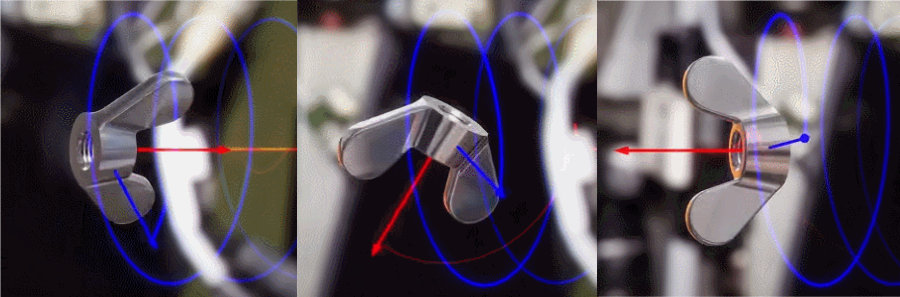
\includegraphics[width=0.9\textwidth]{dzhani.jpg}
\end{center}
   \caption{Джанибековын эффектийг дүрслэн үзүүлэв \cite{28}.}
\label{fig:10}
\end{figure*}

Дэлхийн тэнхлэгийн эргэлтийн гэнэтийн өөрчлөлтийн зарчим нь эргэлдэж буй биетүүдийн физикийн суурь дээр оршдог. Үүний уламжлалт жишээ бол Оросын сансрын нисгэгч Владимир Джанибековын нээсэн Джанибековын эффект бөгөөд Зураг \ref{fig:10}-д дүрслэгдсэн байна \cite{37}. Эргэлтийн инерцийн гурван гол тэнхлэгийн аль нэг дээрээ төгс эргэхгүй байгаа биет нь тогтвортой эргэлтийн тэнхлэгийг хадгалахгүй. Хэрэв тухайн биет хоёр дахь гол тэнхлэгийнхээ дагуу эргэлтэнд ойртсон байвал эргэлтийн чиглэл нь гэнэт өөрчлөгдөж байгаа мэт санагдах хөдөлгөөнтэй болно. Хэдийгээр энэ нь Дэлхийн түргэн эргэлтийг бидний төсөөлдөгтэй яг ижил биш ч, гадаад хүчний нөлөөгүй нөхцөлд зөвхөн эргэлтийн физик нь Дэлхийн эргэлтийн тэнхлэгийн гэнэтийн өөрчлөлтийг тайлбарлаж чадна.

Яг нарийн ярих бол Дэлхий яг ийм энгийн ба жигд Джанибековын эффектэд ордоггүй гэдэг нь бараг тодорхой юм. Хэрвээ тийм байсан бол бид Дэлхийн эргэлтийн тэнхлэгийн аажим өөрчлөлтийг цаг хугацааны турш илрүүлж чадна. Харин бидний үзэж байгаагаар бол Дэлхийн физикийн бүтцэд тодорхой давтамжтай, гэнэтийн тасалдал гарч, түүний “гадна эргэлтийн” (царцдас/мандал) болон “дотоод эргэлтийн биетүүд” (газар доторх цөм) сална гэж үздэг. Гадаад хүчин зүйлгүйгээр өнцгийн импульсийг хадгалах хууль ёсоор Дэлхий эргэлтийн тэнхлэгээ гэнэт сольж чадахгүй; тиймээс гадна болон дотоод эргэлтийн биетүүдийн салалт нь дэлхийд гаднын цохилт үүсээгүй тохиолдолд эргэлтийн гэнэтийн солигдлыг үүсгэж болох цөөн зүйлсийн нэг юм.

Дэлхийн доторх тасалдлыг өдөөдөг тодорхой процесс нь Дэлхийн цөмийг бүрдүүлдэг төмрийн бүтцийн фазын өөрчлөлт гэж үздэг (Зураг \ref{fig:11}). Дотоод цөм нь зургаан өнцөгт нягт багцалдсан төмрөөс (Fe) бүрддэг \cite{141}. Энэ hcp-Fe нь шингэн металл төлөв рүү шилжихэд кинетик энерги ялгаруулж, гадаад цөм рүү шилжинэ. Энэ фазын өөрчлөлт нь цөмийн соронзон нэвчимтгий чанарыг бууруулж, гадаад соронзон оронг сулруулж, дулаан ялгаруулдаг бөгөөд ингэснээр мандалд LLVP (том хэмжээний бага хурдтай хярын муж) бүтцүүд үүсэхэд \cite{38}, Далайн ёроолын хэт гүн давхаргаар дамжин Дэлхийн гадарга руу дулаан хүргэгдэнэ (Зураг \ref{fig:12}). Эдгээр чиг хандлагуудыг сүүлийн хэдэн зуунд сайн баримтжуулсан бөгөөд энэ өгүүлэлд цаашид авч үзэх болно.

\begin{figure*}[t]
\begin{center}
% \fbox{\rule{0pt}{2in} \rule{.9\linewidth}{0pt}}
\includegraphics[width=1\textwidth]{layers.jpg}
\end{center}
   \caption{ECDO эргэлтийн өөрчлөлтөд хүргэдэг Дэлхийн дотоод процессуудыг дүрслэн үзүүлэв \cite{129}.}
\label{fig:11}

\end{figure*}


\begin{figure}[t]
\begin{center}
% \fbox{\rule{0pt}{2in} \rule{0.9\linewidth}{0pt}}
   \includegraphics[width=1\linewidth]{llvp.jpg}
\end{center}
   \caption{Өмнөд Африкийн доорх LLVP-ийн дэлгэрэнгүй дүрслэл \cite{28}.}
\label{fig:12}
\label{fig:onecol}
\end{figure}


Дэлхийн дотор энэ процесс эсрэгээр өрнөдөг бөгөөд үүний үр дүнд эргэлтийн өнөөгийн төлөв рүү буцаж шилжих үйл явц тийм ч удалгүй явагддаг гэж үздэг.

\section{Дэлхийн ойрын ирээдүйн эргэхийн нотолгоо}

Бид дахин нэг удаа Дэлхий эргэхийн ирмэг дээр байгаа гэдэгт хүчтэй үндэслэл бий. Сүүлийн хэдэн мянган жилд мөхөл сүйрэл болоогүй бөгөөд энэ нь түүхэн тэмдэглэл, өгөгдөлд үндэслэн ийм үйл явдал давтагддаг давтамж юм. Дахин эргэх гэж байгааг баталж буй хамгийн хүчтэй нотолгоо нь сүүлийн үеийн геомагнитийн мэдээллүүд бөгөөд эдгээр нь Дэлхийн геомагнитийн талбай ойролцоогоор хоёр мянган жилийн турш сулардсаар ирснийг харуулж байна. Энэ сулралт улам хурдсаж, сүүлийн хэдэн арван жилд аюултай түвшинд хүрсэн байна.
Depicted in Figure \ref{fig:14} нь 1590 болон 2025 оны Дэлхийн геомагнитийн орныг харуулж байна \cite{125,126}. Зурагт үзүүлснээр, уг орон мэдэгдэхүйц суларсан байна.

Геомагнитийн орон суларч байгаа өөр нэг үзүүлэлт нь геомагнитийн умард туйлын байршил юм (Зураг \ref{fig:13}). Геомагнитийн умард туйл түүхэн туршид Канадын Арктикт байжээ. Гэвч сүүлийн хэдэн зууны турш аажим шилжиж ирсэн бөгөөд хэдэн арван жилийн өмнөөс энэ хөдөлгөөн эрс хурдассан. Одоо жилд 55 км-ийн хурдтайгаар Оросын зүг рүү түргэн шилжиж байна \cite{124}.

\begin{figure*}[t]
\begin{center}
% \fbox{\rule{0pt}{2in} \rule{.9\linewidth}{0pt}}
\includegraphics[width=0.9\textwidth]{saa.jpg}
\end{center}
   \caption{1590 оноос 2025 он хүртэлх геомагнитийн орны суларлыг харуулсан зураг. gufm1 болон IGRF-14 загварууд ашигласан \cite{125,126}.}
\label{fig:14}
\end{figure*}

\begin{figure}[t]
\begin{center}
% \fbox{\rule{0pt}{2in} \rule{1\linewidth}{0pt}}
   \includegraphics[width=1\linewidth]{npw.jpg}
\end{center}
   \caption{1590-2025 оны хоорондох геомагнитийн умард туйлын байршлыг 5 жилээр дүрслэн харуулсан \cite{142}.}
\label{fig:13}

\label{fig:onecol}
\end{figure}

\begin{figure}[t]
\begin{center}
% \fbox{\rule{0pt}{2in} \rule{1\linewidth}{0pt}}
   \includegraphics[width=1\linewidth]{ocean-highlight.jpg}
\end{center}
   \caption{Гүн ($>$2000 м гүн) далай тэнгисийн дулаарлын хурд 1991–2010 онд, улаанаар тойруулсан \cite{132}.}
\label{fig:15}
\label{fig:onecol}
\end{figure}

Дэлхийн соронзон орон дотоод динамоор үүсдэг гэж үздэг — Дэлхийн гадаад цөм дотор эргэх хөдөлгөөнөөс үүдэлтэй магмын урсгалын дугуй баганууд \cite{123}. Соронзон орны сулрал нь Дэлхийн гүнд болсон эмгэгийн шинж тэмдэг юм. ECDO онолын дагуу эдгээр эмгэгүүд нь дулаан ялгаруулж, эцэст нь дэлхийн хуулийн болон цөмийн хооронд тусгаарлалт үүсгэж, улмаар дэлхий эргэхэд хүргэдэг \cite{1}.

Дотоод гүнээс дулаан ялгаруулдаг процессуудыг батлах олон тооны мэдээлэл бий. Дэлхий дулаарч байгааг эх газрын болон далайн гадаргын температурын өсөлт \cite{127,128}, дэлхийн дулааны багануудтай хосолсон агаар мандлын CO2 түвшний өсөлт \cite{129,130}, мөн дэлхийн мөсний талбайн бууралт \cite{131} харуулж байна. Эдгээр мэдээлэл нь CO2-ийн өсөлт болон дулаарал нь "хүний гаралтай" уур амьсгалын өөрчлөлтийн шалтгаан биш харин, дотоод цөмийн дулаан ялгаруулалтын үр дагавар болохыг харуулж байна \cite{129}.

Хамгийн чухал нь, гүн далайн (гүн $>$2000 м) дулаарал судлахад зөвхөн далайн гүний ус дулаарч байгаа төдийгүй, хамгийн их дулаарал 4000–6000 м-ийн хоорондох абиссаль давхаргад илэрч байна. Энэ дулаан төв нь 4000 метрээс доош байдаг \cite{132,129}, хэрвээ далайг агаар мандлаас дээрээс нь халааж байсан бол ийм зүйл тохиох боломжгүй байв. Ийм өгөгдөл нь манай үеийн уур амьсгал, соронзон орны өөрчлөлтийг Дэлхийн гүн дэх процессууд хөдөлгөж буйн нотолгоо болдог. Зураг \ref{fig:15}-д 1991–2010 оны дэлхийн гүн далайн дулаарлын хурдыг үзүүлсэн байна \cite{132}.

\section{Гэнэтийн Дэлхийн Эргэлтийг Загварчлах}
\begin{figure}[b]
\begin{center}
% \fbox{\rule{0pt}{2in} \rule{1\linewidth}{0pt}}
   \includegraphics[width=1\linewidth]{saa-crop.jpeg}
\end{center}
   \caption{Өмнөд Атлантын Аномалийн цэгүүдэд суурилсан хувьсалтын цэгийн тооцоолол 2059 оны гуравдугаар сарын 13-ны өдрийг зааж байна \cite{125,126}.}
\label{fig:16}
\label{fig:onecol}
\end{figure}

Дэлхийн дараагийн эргэлтийн цаг хугацааг урьдчилан таамаглах нь нарийн төвөгтэй ажил юм. Одоогоор бидний хамгийн сайн загвар бол Дэлхийн геомагнит талбай буюу Өмнөд Атлантын Аномали (ӨАА) юм. Өмнөд Атлантын дээгүүрх энэ бүс нь хамгийн сул геомагнит талбайтай бөгөөд энэ талбай 32,000 нанотеслаас доош хүчтэй хэсгийг хамардаг гэж тодорхойлогддог \cite{135}, энэ нь 1590 онд хэмжигдсэн хамгийн бага утга байв. ӨАА-ийн гадаргуугийн хамрах хүрээ 1590 онд Дэлхийн нийт гадаргуугийн 1\% байсан бол 2025 онд 21\% болж өссөн байна \cite{136}.

Дэлхий 언제 эргэхийг таамаглахын тулд би ӨАА-ийн гадаргуугийн хамрах хүрээний мэдээллийг хүчийн хууль бүхий хувьсалтын цэгийн тэгшитгэлд тааруулж, энэ нь нарийн төвөгтэй систем эгзэгтэй шилжилтийн цэгт хүрэхэд огцом өөрчлөлт гарахыг загварчилдаг. Миний тооцооллоор тухайн хувьсалтын цэгийг 2059 оны гуравдугаар сарын 13-нд гарах магадлалтай гэж гарсан (Зураг \ref{fig:16}). Энэ таамаглал нь шилжилтийн цэгт ойртох тусам улам нарийвчлан тодорхой болох болно \cite{136}.

Эргэлтийн тэнхлэгийн хэлбэлзэл, цаг агаарын гажуудал, газар хөдлөлт болон галт уулын өгөгдөл зэрэг бусад хэмжигдэхүүнүүд нь Дэлхийн дараагийн эргэлт хэзээ болохыг илүү сайн таамаглахад туслах боломжтой.

\section{ECDO-гийн түүхэн цаг хугацааны шугам}

Өнгөрсөн ECDO үйл явдлуудын яг цаг хугацааг тогтоох нь хүндрэлтэй боловч, Голоцен үеийн турш дор хаяж хоёр ECDO үйл явдал болсон байх магадлалтай. Египетийн лам нараас Геродотын дамжуулсан өгүүллэгийн дагуу, \textit{"анхны хаанаас эхлээд сүүлчийн Хефайстосын тахилч хүртэл гурван зуун дөч, нэгэн үе дамжсан... Энэ хугацаанд нар дөрвөн удаа өөрийн хэвшмэл мандахынхаа газраас шилжиж, одоо жаргадаг газраасаа хоёр удаа мандаж, одоо манддаг газраасаа хоёр удаа жаргаж байсан"} \cite{32}. МЭӨ тавдугаар зуунд амьдарч байсан Платон \cite{111} Атлантидыг ганц өдөр, шөнийн дотор сүйрүүлсэн үер болсноос хойш 9000 жил өнгөрөхөд \textit{"олон үер болсон бөгөөд ууланд амь гарсан хүмүүс бичиг үсгээ мэдэхгүй болж, олон үеийн турш амьдрах арга олж авахад бүхнээ зориулсан"} гэж тэмдэглэсэн байна \cite{112}. Энэ нь Бороо ихтэй Дриасын төгсгөл буюу МЭӨ 9700 оноос хойш дор хаяж хоёр удаа эргэх үзэгдэл болсон байж болзошгүйг илэрхийлж байна. Энэ өгүүлэл болон миний судалгаанд \cite{2} дурдсан баримтууд Платоны хэлсэнтэй нийцэж буйг харуулж байна.
The most recent candidate date for an ECDO flip is during the period of 2300 to 1600 BCE, to which many cataclysmic flood accounts (Gun-Yu \cite{113,114,115}, Ogyges \cite{116,117}, Peru \cite{118,119}, Exodus \cite{120}), civilizational destructions and abandonments (Mohenjo-Daro \cite{121}, Minoan Crete\cite{100,101}) and physical anomalies (bond events \cite{122}, 4.2 kiloyear event \cite{90}) have been dated. There is no ample convergence of evidence more recent than this suggesting a major catastrophic event.

\section{Дүгнэлт}

NANOOK ажиллагаа нь Дэлхийн II дайны дараа АНУ-ын Арктик болон Зөвлөлтийн хойд эргийг зураглах зорилготой, Хүйтэн дайны үеийн тагнуулын ажиллагаа байв \cite{137}. Тэдний судалгааны явцад соронзон туйл өмнөх экспедицүүдийн ололтын дагуу байх ёстойгоос 125-200 милийн хойно байрлаж буйг илрүүлжээ. Иймд, \textit{"Засгийн газрын эрдэмтдийн дунд соронзон болон газарзүйн туйл давхацвал юу болох вэ гэсэн асуулт гарсан юм. Үүнд хариу олохын тулд доктор Пол А. Сайплыг төслийн удирдлагаар томилж, Ранд корпорацад давхар бөмбөрцөг загварууд ашиглан судалгаа хийх гэрээ хийсэн – дотоод бөмбөрцөг нь дэлхийн цахилгаанаар цэнэглэгдсэн хайлмаг төмрийн голыг илэрхийлж, түүний тэнхлэг нь “соронзон” туйлуудыг тодорхойлно; гадар бөмбөрцөг нь дэлхийн царцыг илэрхийлж, “газарзүйн” туйлын тэнхлэгэээр эргэнэ. Давтан туршилтаар батлагдсан нь, “соронзон” туйл “газарзүйн” туйлд ойртох үед тодорхой нэг мөчид соронзон туйл төвд тэмүүлэх хүчээр татагдаж буй мэт хурдан давхцаж үсрэн давхацна; гэхдээ туйлууд давхацахын оронд, “соронзон” туйл “газарзүйн” туйлын эргэн тойронд эргэлдэн, хөвөх хүчээр экваторт зүглэж, хоёр тэнхлэгийн ялгаа бараг 89 градус болно. Энэхүү туйлын “эргэлт” болсны дараа тэнхлэгүүд урт хугацааны туршид аажмаар дахин ойртож эхэлнэ"} \cite{138,139}.

Үүний дараа, \textit{"1948 оны эхээр хошууч Уайт Пентагонд болсон нэгэн шинжлэх ухааны хуралд оролцохдоо, эрдэмтэд ойрын хугацаанд тохиох туйл эргэх үзэгдлийн талаар олон нийтэд мэдээлэх нь зүйтэй эсэх тухай хэлэлцжээ. Аль ч эрдэмтэн энэ мэдээллийг олон нийтээс нуухыг зөвшөөрөөгүй; нөгөөтэйгүүр, хэрхэн мэдээлэхийг шийдэж чадахгүй байв. Энэ үзэгдлийн талаархи мэдлэг нийгмийн ёс суртахууны хэм хэмжээг сүйрүүлэх вий гэж зарим нь эмээж байлаа. Гэсэн ч, 1950-иад оны эхээр туйл эргэх үзэгдлийн талаар мэдээлэл сонины булан болон сэтгүүлийн өгүүлэлд гарсан ч гайхмаар нь, алмайрсан, үл итгэсэн, эсвэл явцуу олон нийтээс огт хариу өгөөгүй юм"} \cite{138,139}.

Яагаад бид үүнд анхаарал хандуулахгүй байна вэ? Дэлхий урьд өмнө ингэж эргэсэн гэдэгт итгэх шалтгаанууд хангалттай. Энэ өгүүлэл болон үргэлжлэл нь Дэлхий ингэж эргэж байсан гэдгийг нотлох олон чиглэлийн нотолгооны нягт тоймыг өгч байна, жишээ нь дэлхийн өнцөг булан бүрийн үерийн домог, тивийг хучсан давс ба далайн чулуужсан үлдэгдэл, эртний газарт оршуулсан хонгилоор барьсан орогнол, амьтны үлдэгдэл, катастрофийн геологийн бүс нутгууд гэх мэт. Хүний нас хэдэн зуун мянган жил үргэлжилдэг гэж үздэг ч орчин үеийн түүх ердөө цөөн мянган жилтэй л байна. Зарим үед дэлхий эргэдэг, тивүүд цэвэрлэгдэж, бид эхнээс буюу Чулуун зуунаас дахин эхэлдэг тул эртний түүхээ цөөхөн сүйрлийн домог болгон үлдээдэг гэж бодож болох уу? Хэрэв тийм бол дахин ингэхээс сэргийлэх нь хүн төрөлхтний хамгийн чухал үүрэг байх магадлалтай.

Төгсгөлд нь Платоны бичсэн \textit{Тимеус}-д гардаг, Афины төрийн зүтгэлтэн Солон ба Египетийн тахилч нарын ярианы тэмдэглэлийг хүргэе \cite{140}: \textit{"Нэг удаа, Солон эртний түүхийн талаар ярилцуулах зорилгоор хамгийн эртний домгийг, эхний хүн байсан гэж хэлэгддэг Фороней, Ниобе-тэй холбоотой түүхийг, мөн Үерийн дараах Девкалион, Пирра хоёрын домгийг, амьд үлдсэн, үр удам нь хэрхэн тархсан тухай домгийг ярьж өгөх гэж оролдсон байна. Тэгтэл тахилч, маш хөгшин хүн: “О Солон, Солон, та нар грекчүүд үргэлж хүүхдүүд шиг байдаг: огт хөгшин грек гэж үгүй юм” гэв. Үүнийг сонсоод Солон, “Та яагаад ингээд хэлээд байна вэ?” хэмээж асуухад, тахилч “Та бүхэн сэтгэлээрээ залуу байна. Учир нь та бүхэнд эртний уламжлалаас гаралтай нэг ч итгэл, насажсан нэг ч мэдлэг үгүй. Хэрэв ямар нэг гайхамшигт үйл явдал, их зүйл болж өнгөрвөл тэр нь манайд ч, та нарт ч, бусад газар ч хатуу чанд тэмдэглэгдэж, манай сүмд хадгалагддаг; харин та нар болон бусад нь шинэ бичиг үсэг сурах бүрдээ дахин цоо шинээр эхэлдэг" гэлээ. Үнэндээ, Солон та сая ярьсан угсаа гарвалын домгүүд чинь хүүхдийн үлгэрээс давсан зүйлгүй. Юу гэвэл, эхлээд чи ганцхан үерийг дурсч байна, гэтэл өмнө нь олон удаа ийм явдал тохиосон; мөн эсрэгээрээ, газар дээр хэт халуун, хэт хүйтэн байхгүй газар бүрт хүн төрөлхтний ул мөр байж л байдаг. Хэрэв ямар нэг эрхэм, гайхамшигтай үйл явдал та нарт ч, бидэнд ч, эсвэл бидний сонссон өөр нэгэн газар болсон бол тэр бүхнийг эрт дээр үеэс тэмдэглэн өнөөг хүртэл хадгалдаг; харин та нар болон бусад орнууд бичиг үсэг, соёлын урлагийг дахин дахин шинээр сурч эхэлдэг бөгөөд жил хугацаагаар тасралтгүй циклийн дараа огторгуйгаас ирэх усны үер дахин ирэхэд зөвхөн бичиг үсэггүй, соёлгүй цөөхөн хүн л амьд үлдэж, бүгд шинэ хүүхдийн адил хуучин цагийн мэдлэггүй болдог. Яг үнэндээ, Солон, Атин улсын тухай сая дурдсан угсаа залгамжлалын түүхүүдээ чи ердөө хүүхдийн үлгэрээр мэдэж байна; та нар зөвхөн ганц үерийг мэддэг, харин өмнө нь олон удаа үер болсон. Мөн хүн төрөлхтний хамгийн шилдэг нь та нарын оршин буй газар төрсөн бөгөөд тэр хүмүүсээс та өөрөө ч, өнөөдрийн хот чинь ч гаралтай, гэхдээ олон үе дамжин бичиг үсэг байхгүйгээс мэдээгүй өнгөрчээ. Үнэндээ, хамгийн их устгал болохоос өмнө одоогийн Афины улс хамгийн зоригтой, дайнд мундаг, бусад тал дээр ч маш сайн зохион байгуулалттай байв. Их тансаг урлаг, хамгийн сайн төрийн тогтолцоог бүрдүүлж байжээ. Та нарын оронд Паетон, Нарангийн хүү, эцгийнхээ тэргийг жолоодож чадаагүйгээс газар дээрх бүхнийг шатааж, өөрөө аянганд өртөж үхсэн тухай яригддаг үлгэр ч үнэн хэрэгтээ тэнгэрт эргэж буй биетүүд дэлхий дээрх бүхнийг удаа дараа устгаж буй тухай хуучин мэдлэг дээр тулгуурласан байна. Хэзээ нэгэн цагт уул толгод дээр, өндөр, хуурай газар суугсад илүү хохирч, гол мөрөн, тэнгисийн эрэгт буй хүмүүс илүү аврагддаг. Манайд ч Нил мөрөн биднийг өөр өөр үеүүдэд аврах үүрэгтэй. Харин бурхад газрын усаар цэвэрлэх үед уулын бэлд буй малчид, хоньчид аврагдаж, хот сууринд буй хүмүүс далай руу урсаж явдаг; манайд бол дээрээс ус бууж урсахгүй, харин доороос булаг мэт гардаг. Ийм учраас энд хадгалагдсан зүйлс хамгийн эртнийд тооцогдож байна;}"

Эдгээр тахилч нар мөн Солонд Атлантисын тухай өгүүлжээ: \textit{"Бидний энд яриад буй газрын аманд багтсан бүх зүйл нь нэвтрэхэд хязгаарлагдмал боомт юм; харин тэнд жинхэнэ далай, түүнийг бүслэн орших газар нутаг нь бүрэн утгаараа эх газар гэдгийг хэлж болно. Энэхүү Атлантисын арал дээр хаадын холбоо бүрэлдэж, том хүчтэй холбоо байгуулж, бүх арлыг эзэмшиж, олон арал, эх газрын хэсэгт ноёрхон байжээ; Стрейтийн доторх газарт тэд Ливиас Египет хүртэл, Европийг Тиррени хүртэл захирч байв. Тэгээд бүгд нийлж, нэгэн довтолгоогоор танай улс, манай улс, Стрейтсийн доторх нутгийг боолчлохыг оролдсон. Тэр үед Солон, танай улсын эр зориг, цэрэг дайны ур ухаан нь бүгдэд тодорч, бусад үндэстнүүд орхиж зугтаахад ганцаараа тэмцэж, дайсныг ялж, ялалтын дурсгал босгож эх нутгаа болон биднийг эрх чөлөөтэй болгосон. Гэвч дараа нь аюултай газар хөдлөлт, үер болсон ба нэгэн аймшигтай өдөр, шөнө өнгөрөхөд дайчдын тань ихэнх хэсэг газар доор орж, Атлантисын арал далайд живж, алга болсон"}.

\section{Талархал}

ECDO онолын анхны зохиогч Ethical Skeptic-д түүний гүн гүнзгий утга санаа агуулсан, шинэлэг, суурь бүтээлийг туурвисанд болон дэлхий дахинд дэлгэсэнд баяр хүргэе. Түүний гурамсан бүтээл \cite{1} нь Экзотермик Гол-Цартын Салангид Хөдөлгөөн Жанибековын Осцилляцийн (ECDO) онолын үндсэн эх сурвалж хэвээр бөгөөд миний энд товч дурдсан эсвэл дурдсангаас ч илүү мэдээллийг өөртөө багтаадаг.

Мөн Хүснэгт 1-д байгаа катастрофийн өгөгдлийг боловсруулсан Анкитэд талархал илэрхийлье.
Мэдээж хэрэг, бидний тулгуур болж буй аваргууд болон эдгээр бүх судалгаа, шинжилгээг хийж энэхүү ажлыг боломжтой болгож, хүн төрөлхтөнд гэрэл авч ирэхээр зүтгэсэн хүмүүсэд талархал илэрхийлье.

\clearpage
\twocolumn

\section{Нэмэлт зургууд}


\begin{figure}[H]
\begin{center}
% \fbox{\rule{0pt}{2in} \rule{1\linewidth}{0pt}}
   \includegraphics[width=1\linewidth]{wave.jpg}
\end{center}
   \caption{Хафрe пирамидын доод хэсэг дэх, парабол хэлбэртэй өгөршлийн процесст ойртон харж буй нь \cite{27}.}
\label{fig:19}
\label{fig:onecol}
\end{figure}

\begin{figure}[H]
\begin{center}
% \fbox{\rule{0pt}{2in} \rule{1\linewidth}{0pt}}
   \includegraphics[width=1\linewidth]{star-stone.jpg}
\end{center}
   \caption{Хуфугийн пирамидын нэгэн амсарт сийлсэн оддын газрын зураг \cite{28}.}
\label{fig:20}
\label{fig:onecol}
\end{figure}

\begin{figure*}[t]
\begin{center}
% \fbox{\rule{0pt}{2in} \rule{.9\linewidth}{0pt}}
\includegraphics[width=1\textwidth]{deepsea.jpg}
\end{center}
   \caption{Гүн болон маш гүн далайн халаалтын аномали нь энгийн агаарын далайн халаалтын муруйтай харьцуулсан зураглал. Ерөнхий халаалтын аномалийг NOAA-с авсан \cite{147}, гүн болон маш гүн давхаргын халаалтын тархалтыг Desbruyeres-ийн судалгаагаас авсан \cite{132}, өгөгдөл боловсруулалт ба дүрслэлийг Ethical Skeptic хийсэн \cite{129}.}
\label{fig:21}
\end{figure*}

\begin{figure*}[t]
\begin{center}
% \fbox{\rule{0pt}{2in} \rule{.9\linewidth}{0pt}}
\includegraphics[width=1\textwidth]{sealevel.jpeg}
\end{center}
   \caption{61 станц дээр 75 жилийн турш далайн түвшний хэлбэлзлийн хувьсвар 20\% -аар нэмэгдсэн нь урсгалын хурд ихсэж байгааг харуулж байна. Далайн түвшний хэлбэлзэл огцом нэмэгдэх нь далайн дулааны түрлэгтэй давхцаж байгаа бөгөөд энэ нь дэлхийн далайн гүнээс үүдэлтэй дулаан ихсэлтээс шалтгаалж байж болохыг зааж байна \cite{2,129}.}
\label{fig:22}
\end{figure*}

\begin{figure*}[t]
\begin{center}
% \fbox{\rule{0pt}{2in} \rule{.9\linewidth}{0pt}}
\includegraphics[width=1\textwidth]{co2.jpg}
\end{center}
   \caption{Агаар мандлын CO2 ppm нь сүүлийн 45 жилийн хугацаанд тогтвортой өссөн бөгөөд энэ нь далайн температурын нэмэгдлээс шалтгаалсан байж магадгүй юм. Эх сурвалж: NOAA \cite{148,129}.}
\label{fig:23}
\end{figure*}

\begin{figure*}[t]
\begin{center}
% \fbox{\rule{0pt}{2in} \rule{.9\linewidth}{0pt}}
\includegraphics[width=1\textwidth]{ice.jpg}

\end{center}
   \caption{Дэлхийн тэнгисийн мөсний хэмжээ сүүлийн 45 жилийн хугацаанд буурсаар байна, энэ нь дэлхийн дулаарлаас шалтгаалж байна. Эх сурвалж: ADS \cite{149}.}
\label{fig:24}
\end{figure*}

\clearpage
\twocolumn

{\small
\renewcommand{\refname}{Ишлэлүүд}
\bibliographystyle{ieee}
\bibliography{egbib}
}

\end{document}